\chapter{相关研究}
本章主要介绍实体链接任务、主动学习方法的研究现状。全章总共分为三节,第一节介绍实体链接任务的基本概念、特征描述以及常用的监督学习和无监督学习的处理方法。第二节介绍主动学习的基本概念、常用方法,以及在其它机器学习任务中的应用。最后一节总结本章的主要内容。

\section{实体链接任务}
\subsection{任务描述}
实体链接任务,即在给定包含实体集$E$的知识库和包含指称项集合$M$的文本的前提下,将文本中的每一个指称项$m\in M$链接到知识库中的对应实体$e\in E$。这里所提到的指称项$m$是指文本中的一段字符串序列,称之为命名实体,通常是人名、地名、机构名。一些研究者也将实体链接任务称为命名实体消歧(Named Entity Disambiguation, NED)。按照所处理的语言种类区分,实体链接任务还可分为单语种的实体链接以及跨语种的实体链接\cite{CLELBBTM},本文主要研究英文实体链接任务。

通常,实体链接任务首先需要经过命名实体识别阶段,在该阶段,文本中的人名、地名、机构名等命名实体会被命名实体识别器识别出来,并划分出字符边界。命名实体识别经过几十年的研究,已经有不少成熟的研究成果\cite{RWNERST,NEROEHRTCDA,RHENERCCBEL}。

在工程实现中,也可借助各种开源的命名实体识别工具包,例如Stanford NER\footnote{http://nlp.stanford.edu/ner/}、OpenNLP\footnote{http://opennlp.apache.org/}、LingPipe\footnote{http://alias-i.com/lingpipe/}等。由于命名实体识别并非本文重点,这里不再赘述。

\begin{figure}[!htb]
	\centering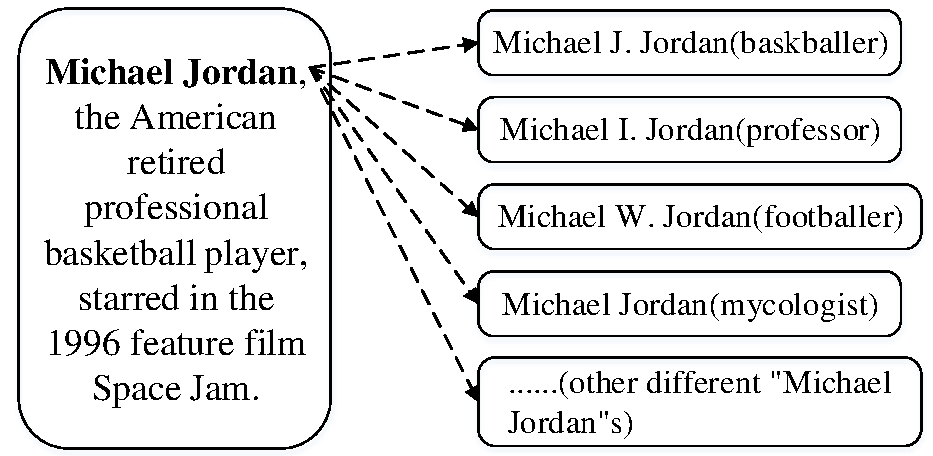
\includegraphics[height=5cm]{resource/el_example}
	\caption{实体链接任务的一个例子,文本中粗体标志的就是指称项。}
	\label{fig:el_example}
\end{figure}

图\ref{fig:el_example}展示了实体链接任务的一个例子。图中左侧是包含指称项“Michael Jordan”的文本,图中右侧是指称项“Michael Jordan”在知识库中可能指向的具体实体,例如NBA球星\textit{Michael J. Jordan}、伯克利机器学习教授\textit{Michael I. Jordan}、足球运动员\textit{Michael W. Jordan}、菌类学家\textit{Michael Jordan}等。实体链接系统需要借助指称项上下文与候选实体在知识库中文本的相似度等特征,将指称项链接到其对应的目标实体。在该例子中,目标实体就是NBA球星\textit{Michael J. Jordan}。

一般来说,实体链接系统分为以下两个模块:
\begin{itemize}
	\item {候选实体生成模块
	
在这个模块中,实体链接系统会为文本中包含的每个指称项$m \in M$生成出它在知识库中可能指向的候选实体集$E_m$。经过多年的研究,研究者已经提出了大量候选实体生成方法。
}
	\item {候选实体排序模块
	
	该模块是实体链接系统中最重要的模块。在大多数情况下,指称项$m$都会对应多个候选实体$e\in E_m$。实体链接系统需要从指称项$m$的候选实体集$E_m$中选出可能性最大的目标实体$e^*$。处理候选实体排序的方法很多,可以划分为有监督学习方法和无监督学习方法。
}
\end{itemize}

\subsection{候选实体生成}\label{section:candidate_generate}
候选实体生成的方法很多,Hachey等人\cite{EELWW}认为能否生成包含目标实体的候选实体集对实体链接的成功与否至关重要。目前在实体链接领域中,使用最广泛的候选实体生成方法是基于词典的候选实体生成方法。

基于词典的候选实体生成方法被多种实体链接系统\cite{CELWTGBM,ELFEEKB}所采纳。以Wikipedia为例,该方法抽取了知识库中实体页(Entity pages)、重定向页(Redirect pages)、消歧页(Disambiguation pages)、文本超链接(Hyperlinks in articles)等结构化信息,通过这些信息构建了离线形式的词典$D$,该词典$D$包含了指称项和指称项可能指向的候选实体。这里的指称项是知识库中实体的多种表述,可以是实体的标题名、缩写名、别名、拼写名等。

实质上,词典$D$即键值对$\left\langle key,value\right\rangle $的集合,其中$key$列是指称项$k$,$value$列是指称项$k$对应的候选实体集$k.value$。本文可以借助Wikipedia知识库中的以下特征抽取得到词典$D$:

\begin{itemize}
	\item {实体页(Entity page)
		
		知识库中每一个实体都包含一个描述该实体的实体页,通常,这个实体页的标题就是该实体被最常用来表述的名字,例如实体页标题“Michael Jordan”就可以用来表示前NBA公牛队球员\textit{Michael Jordan}这个实体。在这个例子里,标题$k=“Michael\, Jordan”$被添加到词典$D$的$key$这一列,对应的实体$k.value=“Michael\, Jordan”$被添加到词典$D$的$value$这一列。
		}
	\item {重定向页(Redirect page)
		
		在很多情况下,不同的表述可能指向同一个实体,对于这类情况,知识库会采用重定向的方式来处理。例如,对于标题为“Michael Jeffrey Jordan”的实体页,会重定向到标题为“Michael Jordan”的实体页。在此例中,标题$k=“Michael\text{\ }Jeffrey\text{\ }Jordan”$被添加到词典$D$的$key$这一列,对应的实体$k.value=“Michael\, Jordan”$被添加到词典$D$的$value$这一列。
	}
	\item {消歧页(Disambiguation page)
		
		在知识库中,不同的实体可以使用相同的表述。消歧页用来展示某个实体表述可以指向的实体集。例如,“Michael Jordan”这个实体表述,在消歧页“Michael Jordan(disambiguation)”中,包含13个指向不同人物的实体,有NBA球员、足球运动员、机器学习教授、爱尔兰政治家等。在这个例子里,标题$k=“Michael\, Jeffrey\, Jordan”$被添加到词典$D$的$key$这一列,对应的13个实体$k.value$被添加到词典$D$的$value$这一列。
	}
	\item {文本超链接(Hyperlinks in articles)
		
		知识库的文本中一般都会包含很多指向其它实体页的超链接,这些超链接的锚文本通常是所链接到的实体的标题或者别名。这类锚文本可以作为目标实体的一种指称项表述。例如,在“Chicago Bulls”这个实体对应词条的文本中,包含这样一段文本,“For his efforts, \textbf{Jordan} was named NBA Most Valuable Player.”,加粗的文本“Jordan”有指向实体页“Michael Jordan”的超链接。在这个例子里,标题$k=“Jordan”$被添加到词典$D$的$key$这一列,对应的实体$k.value=“Michael\, Jordan”$被添加到词典$D$的$value$这一列。
	}
\end{itemize}

\begin{table}[!htb]
	\caption{候选实体词典的例子\label{tab:candidate_dict_example}}
	\begin{center}
		\begin{tabular}{|c|c|}
			\hline
			$k$(Name) & $k.value$(Entity) \\ \hline
			\multirow{6}{*}{Michael Jordan} &  \textit{Michael Jordan}\\
			& \textit{Michael Jordan (footballer)} \\
			& \textit{Mike Jordan (racing driver) } \\
			& \textit{Michael I. Jordan} \\
			& \textit{Michael Jordan (Irish politician)} \\
			& ... ... \\
			\hline
		\end{tabular}
	\end{center}
\end{table}

通过以上的几种方式,可以构建出候选实体词典$D$。在后续阶段,只要给出指称项$m$,实体链接系统就能通过查找词典的方式得到$m$对应的候选实体集$E_m$。表\ref{tab:candidate_dict_example}是候选实体词典中指称项为“Michael Jordan”的一个例子,根据$k$列的指称项,可以在词典$k.value$列中查到“Michael Jordan”对应的所有可能指向的候选实体。一般来说,为了提高实体链接系统的性能,需要尽可能保证目标实体被包含在候选实体集中。

\subsection{候选实体排序}\label{section:candidate_rank}
对于给定的指称项$m$,通过基于词典的候选实体生成方法获得候选实体集$E_m$后,候选实体集$E_m$一般包含多个候选实体,即$|E_m|>1$,例如“Michael Jordan”这个指称项对应的候选实体集就包含\textit{Michael Jordan}、\textit{Michael Jordan (footballer)}、\textit{Mike Jordan (racing driver) }等多个候选实体。Shen等人\cite{ELKBITS}通过调研发现,TAC-KBP2010数据集中平均每个指称项指向12.9个候选实体,TAC-KBP2011数据集中平均每个指称项指向13.1个候选实体。实体链接系统需要对$E_m$中的候选实体做排序,将排序最靠前的实体作为最佳预测实体。候选实体排序模块是实体链接系统中的重要模块。研究者对候选实体排序方法在监督学习方法和无监督学习方法中均有做相关工作。

\setcounter{secnumdepth}{3}
\subsubsection{二分类法}
二分类法(Binary Classification Methods)是处理实体链接任务中候选实体排序问题的一种简单高效的有监督学习方法。在给定一个指称项$m$和其对应候选实体集中的某一个候选实体$e_i\in E_m$的样本对$\left\langle m,e_i\right\rangle $后,候选实体排序模块的工作是判断$e_i$是否为$m$的目标实体。如果$e_i$是$m$的目标实体,则将样本对$\left\langle m,e_i\right\rangle $划分为正例,否则将其划分为反例。

对于给定的样本对$\left\langle m,e_i\right\rangle $,需要通过特征提取算法提取特征向量,然后将该向量作为模型的输入,模型的输出为样本的分类类型,即正例和反例。在基于二分类法的候选实体排序模型的训练阶段,需要提供足够的带标注的样本对$\left\langle m,e_i\right\rangle $作为训练集,如果$e_i$就是目标实体,则标注为正例,否则标注为反例。当完成模型训练以后,给定未标注的样本对$\left\langle m,e_i\right\rangle $,提取特征输入训练好的模型,模型返回分类结果,根据输出结果是正例还是反例判断$e_i$是否是$m$的目标实体。

二分类法的模型有很多种选择。Xiaohua等人\cite{ELFT}、Jinlan等人\cite{ELNDUSCM}、Yahui等人\cite{FNEDLSBKB}使用支持向量机模型(Support Vector Machine, SVM)来处理二分类的实体链接问题。支持向量机是一种特征空间上的间隔最大化的分类器。另外,支持向量机的核函数(Kernel Function)能够将非线性可分的输入映射到高维线性可分的特征空间。大量研究表明,支持向量机特别适合处理二分类问题。其它可用于处理二分类问题的模型还包括朴素贝叶斯模型(Naive Bayes)、逻辑斯谛回归模型(Logistic Regression)、K-近邻模型(K-Nearest Neighbors)等。

\subsubsection{排序学习法}
排序学习法(Learning to Rank Methods)也是一种用于处理实体链接任务的监督学习方法,该方法最早被用来解决信息检索领域中的网页排序(Page Rank)问题。相比于二分类法,排序法克服了二分类法训练样本集正例、反例数量不平衡的问题,另外,当某个指称项的多个候选实体样本对都被判断为正例时,需要通过其它方法从这些候选实体中选出最有可能是目标实体的实体。与二分类法不同,排序学习法会对给定指称项对应的所有候选实体进行评分,然后根据评分对候选实体进行排序,最后选择评分最高的候选实体作为预测的目标实体。排序学习法主要可以分为三种方法,分别是基于数据点的方法(Pointwise)、基于数据对的方法(Pairwise)和基于列表的方法(Listwise)。

\begin{itemize}
	\item {基于数据点的方法
		
		David等人\cite{SRUR}将基于数据点的方法用于网页排序任务。在实体链接任务中,基于数据点的方法会以候选实体为粒度,对指称项$m$和其中一项候选实体$e_i\in E_m$的链接置信度进行计算。模型的输入是单个候选实体样本对$\left\langle m,e_i\right\rangle $,模型的输出可以是回归值,也可以是分类值。例如,对于$\left\langle m,e_i\right\rangle $,如果输出的是回归值评分,则选出$e_i\in E_m$中评分最高的候选实体作为预测目标实体。
		
		\begin{table}[!htb]
			\caption{Pointwise模型的例子\label{tab:piontwise}}
			\begin{center}
				\begin{tabular}{|c|c|c|}
					\hline
					\multirow{2}{*}{} & \multicolumn{2}{c|}{基于数据点的方法} \\ \cline{2-3}
					& 回归 & 分类 \\ \hline
					输入空间 & \multicolumn{2}{c|}{$\left\langle m,e_i\right\rangle $} \\ \hline
					输出空间 & 实数 & 分类 \\ \hline
					Hypothesis Space & \multicolumn{2}{c|}{评分函数 $f(\left\langle m,e_i\right\rangle)$} \\ \hline
					\multirow{2}{*}{损失函数} & 回归损失 & 分类损失 \\ \cline{2-3}
					& \multicolumn{2}{c|}{$L(f;\left\langle m,e_i\right\rangle,y_j)$} \\ \hline
				\end{tabular}
			\end{center}
		\end{table}
	
	如表\ref{tab:piontwise}所示,对于回归值来说,无论是线性回归还是逻辑斯蒂回归,最后的输出都是一个实数,并可以对每个候选实体对应的实数进行排序。对于分类值来说,可以得出无序的实体类别及其置信度,即该实体是不是目标实体,以及是目标实体的置信度。
	}
	\item {基于数据对的方法
		
		与基于数据点的方法不同,基于数据对的方法以指称项的候选实体对为粒度,对指称项$m$及其候选实体对$e_i\in E_m$和$e_j\in E_m$的链接置信度进行计算。模型的输入是由指称项和两个候选实体构成的三元组$\left\langle m,e_i,e_j\right\rangle $。模型的输出是一个二分类标签。例如,当候选实体$e_i$比候选实体$e_j$更接近目标实体时,模型输出为1,反之则模型输出为-1。基于数据对的方法包括RankBoost\cite{AMIRSBOR}、RankSVM\cite{ESLRES}、RankNet\cite{ADRFPS}。
		
		%\begin{figure}[!htb]
		%	\centering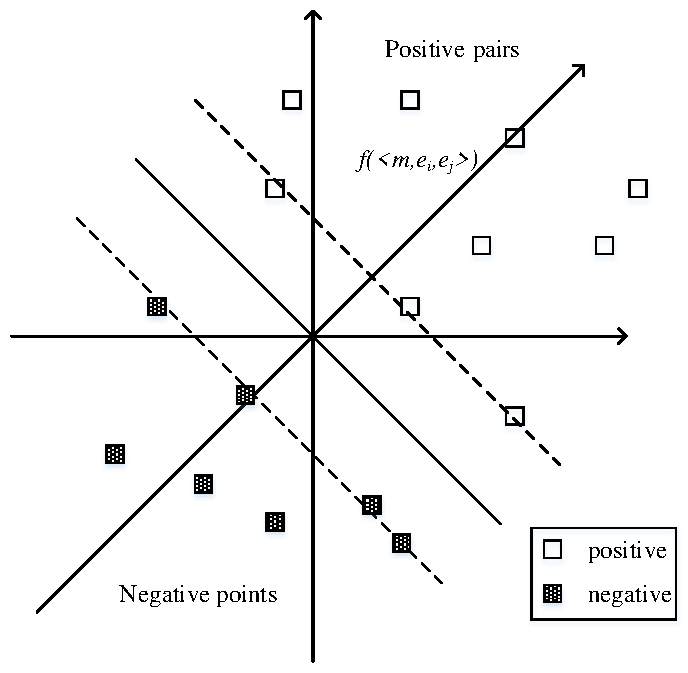
\includegraphics[height=9cm]{resource/pairwise}
		%	\caption{基于支持向量机的pairwise模型示意图}
		%	\label{fig:pairwise_example}
		%\end{figure}
	}
	\item {基于列表的方法
		
		基于列表的方法不再单独考虑某一个候选实体或者某一对候选实体,而是同时考虑一组候选实体,主要通过直接优化候选实体的评价方法和定义损失函数两种方法实现。基于列表的方法的主要模型包括:AdaRank\cite{xu2007adarank}、SVM-MAP\cite{yue2007support}、ListNet\cite{LTRFPATLA}、LambdaMART\cite{burges2010ranknet}等。
		
		Cao等人\cite{LTRFPATLA}提出ListNet来描述Listwise的损失函数,该损失函数的定义是模型计算所得的候选实体排序和真实候选实体排序之间的差异程度,训练过程中通过算法将该差异最小化。训练完毕得到模型后,将候选实体排序问题转化为概率分布问题,用“交叉熵”来衡量计算得到的候选实体与真实排序的差异,通过最小化该差异来完成排序任务。
	}
\end{itemize}

\subsubsection{基于图的协同推断}
Han等人\cite{CELWTGBM}提出的基于图的协同推断方法(Collective Graph-Based Methods)是一种用于处理实体链接任务的无监督学习方法。该方法不仅考虑到了单个指称项和候选实体的上下文相似度,并将其作为局部相似度,还基于同一文档内不同指称项指向的实体具有关联性这一特点,借助知识库中实体的链接关系,综合考虑了实体之间的语义关联度,并将其作为全局相似度。在这两种相似度的基础上,构造用有向图表示的推理图,并基于图的协同推断方法处理候选实体排序问题。

构造出推理图后,可以通过协同推断算法,利用图模型中的随机行走(Random Walk)算法\cite{tong2006fast}来确定同一文档中的各个指称项对应的最佳候选实体。Han等人\cite{CELWTGBM}的实验表明,综合考虑了全局相似度这一特征后,在IITB数据集\footnote{http://www.cse.iitb.ac.in/~soumen/doc/}上实验得到的F1值是73\%,实体链接系统性能得到了显著提升。

\subsection{评测资源}
评测资源主要由知识库和文本语料构成。本节将介绍目前可用的实体链接任务相关评测资源。

(1)目前在实体链接任务中常用的知识库主要如下:
\begin{itemize}
	\item 维基百科\footnote{http://www.wikipedia.org}。该知识库是由非营利组织维基媒体基金会负责营运。2015年11月英文版维基百科包含400万个实体,包括832000个人物、639,000个地点、209,000个机构等。
	\item Knowledge Graph\footnote{https://www.google.com/intl/es419/insidesearch/features/search/knowledge.html}。该知识库当前最新版本大约包含5.7亿个实体。
	\item TAC会议的KBP任务发布的基于维基百科的知识库,大约包含818741个实体。
\end{itemize}

(2)目前在实体链接任务中常用的评测语料库主要如下:
\begin{itemize}
	\item AIDA\cite{hoffart2013discovering}。该数据集的语料来自英文新闻文本,并在CoNLL'03\cite{tjong2003introduction}的基础上做了实体链接标注。数据集包含 1393 篇文章,34956 个指称项目,但是 6141 个指称项对应的实体无法与维基百科词条对应,因此可用指称项个数为28815个。
	\item TAC-KBP2010\cite{ji2010overview}发布的实体链接语料库。该语料主要来源于英文新闻以及Web文本,主要包含人物指称项1877个,机构指称项3960个,地理政治指称项1817个。
\end{itemize}

\section{主动学习}
监督学习模型被广泛用于分类问题,但是所有基于监督学习的分类模型都需要使用带标注的样本集对模型进行训练。对未标注的样本进行人工标注费时费力,并且训练样本可能存在重复,因此没有必要对这类样本做重复标注。主动学习能够根据学习进程,选择最佳学习样本交由人工标注。主动学习的样本选择过程主要分为两个阶段,分别是初始训练样本选择阶段和迭代训练样本选择阶段。

%\begin{figure}[!htb]
%	\centering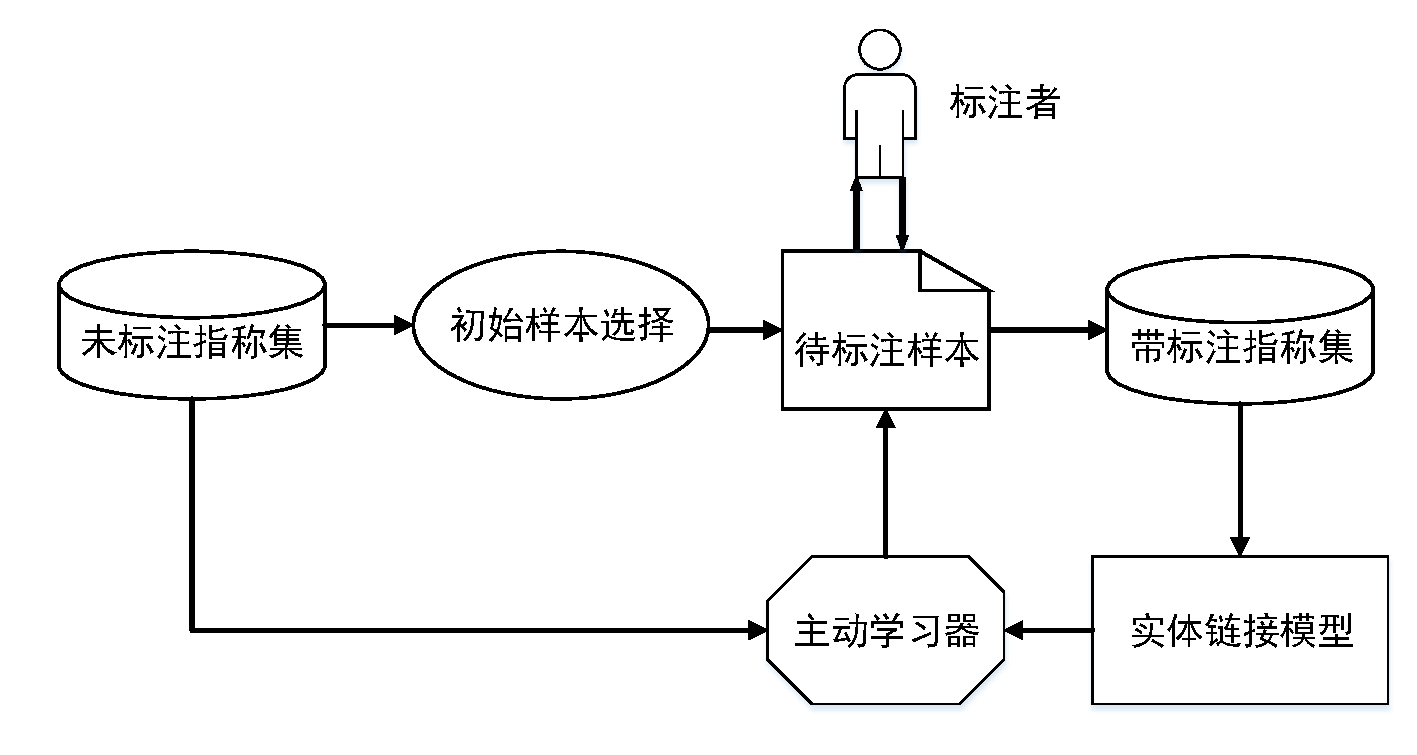
\includegraphics[height=7cm]{resource/al_overview}
%	\caption{主动学习流程概览}
%	\label{fig:al_overview}
%\end{figure}

第一阶段,主动学习器构造一个规模较小的初始带标注的样本集,用于训练一个初始模型。第二阶段,在模型迭代训练过程中,主动学习器能主动选择包含信息量大的未标注样本交由专家标注,然后将这些带标注的样本加入到训练集, 从而在保证模型泛化能力的同时,减小人工标注的工作量。

\subsection{基于不确定度的样本选择策略}\label{sec:al_single}
基于不确定度的主动学习算法采用了不确定度采样(Uncertainty Sampling)的方式选择待标注样本。该采样方式由Lewis等人\cite{lewis1994heterogeneous}于1994年提出,基于最大化人工标注效率的原则,尽量选择因置信度较小而更可能被错误分类的样本点,交由人工标注,以此加快模型的训练速度。

以基于SVM的二分类问题为例,样本点$x_i$到分类超平面的距离可由公式\ref{eq:svm_dis}计算:

\begin{equation}\label{eq:svm_dis}
f(x_i)=\sum_{j=1}^{n}\alpha_j y_j K(x_j,x_i)+b
\end{equation}

公式\ref{eq:svm_dis}中$K(x_j,x_i)$是SVM的核函数,代表样本点$x_i$和样本点$x_j$的相似度。根据样本点到分类超平面的距离,可以预测样本分类的置信度。离分类超平面越近,分类置信度越低,越容易被主动学习器选中。反之,则分类置信度越高,越不容易被主动学习器选中。

%\floatname{algorithm}{算法}
%\renewcommand{\algorithmicrequire}{\textbf{输入:}} % Use Input in the format of Algorithm
%\renewcommand{\algorithmicensure}{\textbf{输出:}} % Use Output in the format of Algorithm
%\begin{algorithm}[!htb]
%	\caption{基于池的主动学习算法}
%	\label{algorithm_pool_based_al}
%	\begin{algorithmic}[1] %这个1 表示每一行都显示数字
%		\REQUIRE ~ %算法的输入参数:Input
%		未标注的样本集$ \mathcal{U}=\{m^{(u)} \}_{u=1}^U $
%		\ENSURE ~ %算法的输出:Output
%		监督学习分类器$\theta$
%		\STATE 从未标注训练集$\mathcal{U}$中选择并标注初始训练样本集$\mathcal{L}_0$\label{al_al_line1}
%		\STATE 利用初始训练样本集$\mathcal{L}_{0}$训练得到弱分类器$\theta=train(\mathcal{L}_{0})$\label{al_al_line2}
%		\REPEAT \label{al_al_line3}
%		\STATE 从$\mathcal{U}$中找出$k$个不确定度最大的样本组成样本集$ \mathcal{U}_{selected} = \{m^{(u)} \}_{u=1}^{k} $\label{al_al_line4}
%		\STATE 对$ \mathcal{U}_{selected}$中的样本进行人工标注得到$ \mathcal{L}_{selected} = \{\left\langle m,e\right\rangle^{(l)} \}_{l=1}^{k} $
%		\STATE $ \mathcal{U} = \mathcal{U} \setminus \mathcal{U}_{selected} $
%		\STATE $ \mathcal{L}_{t+1} = \mathcal{L}_{t} \cup \mathcal{L}_{selected} $
%		\STATE $\theta=train(\mathcal{L}_{t+1})$
%		\UNTIL {达到预期精度或样本集已全部标注} \label{al_al_line9}
%	\end{algorithmic}
%\end{algorithm}

基于池的主动学习方法\cite{muslea2006active}在目前研究中使用最为广泛。该方法的关键步骤是,在待标注样本选择的过程中设计算法对未标注样本的信息量进行定量分析。对于二分类问题来说,距离分类超平面最近的样本点就是分类置信度最接近0的样本点,这些样本点的分类不确定度相对较高。但是对于分类标签个数大于2的多分类问题来说,仅根据分类置信度是否接近0已无法区分样本的不确定度。对于多分类问题来说,不确定度的度量方式主要有三种。

(1)置信度。基于置信度的不确定度度量方式是用于度量不确定度最基本的方式。对于某一个样本点,其对应的所有可能的分类标签都会被赋予相应的置信度,将其中置信度最大的标签作为预测最佳标签,并将此标签的置信度作为该样本被正确分类的置信度。

\begin{align}\label{eq:al_least_confident}
\begin{aligned}
x_{LC}^*&=\argmin_x P_\theta(\hat{y}|x)\\
&=\argmax_x 1-P_\theta(\hat{y}|x)
\end{aligned}
\end{align}

在公式\ref{eq:al_least_confident}中,$y^*=\argmax_y P_\theta (y|x)$,即在当前分类器$\theta$下,样本$x$的最佳预测分类标签。基于该度量方式,最佳预测分类标签的置信度越低,则分类的不确定度越高,这些样本点更应该被选择出来进行人工标注。该度量方式可由0-1损失(0-1 loss)来解释。该度量方式的缺点是只考虑了最佳分类标签的置信度,而丢弃了其他分类标签的置信度的分布情况。

(2)间隔。基于间隔的不确定度度量方式以最佳预测分类标签置信度和次佳预测分类标签置信度的差值作为考量因素。

\begin{align}\label{eq:al_margin}
\begin{aligned}
x_M^*&=\argmin_x [P_\theta(y^{*1}|x)-P_\theta(y^{*2}|x)]\\
&=\argmax_x [P_\theta(y^{*2}|x)-P_\theta(y^{*1}|x)]
\end{aligned}
\end{align}

在公式\ref{eq:al_margin}中,$y^{*1}$和$y^{*2}$分别是在当前分类器$\theta$下,样本$x$的最佳预测分类标签和次佳预测分类标签。该度量方式通过同时考虑两个分类标签的置信度,在一定程度上克服了前一种度量方式的缺点。基于该度量方式,间隔越大的样本点,分类器越容易从最佳的两个分类标签中区分出最佳预测样本点,这种样本的分类置信度就较高。因此,主动学习器应该选择间隔较小的样本点,这些样本点的分类置信度较低,对模型的训练更有帮助。

(3)熵值。在主动学习方法中,目前使用较广泛的不确定度度量方式是熵值度量法,熵是用来描述模型对样本点分类时,分类结果混乱程度的一项指标。熵值的计算方法如公式\ref{eq:al_entropy}所示。

\begin{align}\label{eq:al_entropy}
\begin{aligned}
x_M^*&=\argmax_x H_\theta (Y|x)\\
&=\argmax_x -\sum_{y}P_\theta(y|x)\log P_\theta(y|x)
\end{aligned}
\end{align}

通过公式\ref{eq:al_entropy},可以看出,基于熵值的不确定度度量方式考虑了样本点$x$对应的所有可能的分类标签的分类置信度,从而使该方法可以描述样本分类结果的整体分布情况。对基于熵值的不确定度度量方式可以由对数损失(Logarithmic Loss)来解释。熵值越大的样本点,分类标签置信度的分布越混乱,样本点的分类不确定度越大。反之,分类标签置信度的分布越集中。极端情况,某一分类标签的置信度为1,其他分类标签的置信度均为0,则熵值为0,这时候分类不确定度是最低的。因此,主动学习器应该选择熵值较大的样本点对模型进行重训练。

\subsection{基于委员会的主动学习算法}
与基于单个模型的主动学习算法不同,Seung等人\cite{freund1997selective}提出的基于委员会的主动学习算法会选择一定数量的分类模型,组成分类委员会。在待标注样本选择过程中,委员会中的各个模型分别对样本点进行分类。各委员会模型分类预测结果最不一致的样本点就是分类不确定度最高的样本点,主动学习器需要选择这些样本点进行人工标注并将其加入训练集对委员会中的所有模型进行重训练。

%\floatname{algorithm}{算法}
%\renewcommand{\algorithmicrequire}{\textbf{输入:}} % Use Input in the format of Algorithm
%\renewcommand{\algorithmicensure}{\textbf{输出:}} % Use Output in the format of Algorithm
%\begin{algorithm}[!htb]
%	\caption{基于委员会的主动学习算法}
%	\label{algorithm_committee_al}
%	\begin{algorithmic}[1] %这个1 表示每一行都显示数字
%		\REQUIRE ~ %算法的输入参数:Input
%		未标注的样本集$ \mathcal{U}=\{m^{(u)} \}_{u=1}^U $
%		\ENSURE ~ %算法的输出:Output
%		监督学习分类器集合$\mathcal{C}=\{\theta_1,\theta_2,...,\theta_n\}$
%		\STATE 从未标注训练集$\mathcal{U}$中选择并标注初始训练样本集$\mathcal{L}_0$
%		\STATE 利用初始训练样本集$\mathcal{L}_{0}$训练得到弱分类器集合$\mathcal{C}=train(\mathcal{L}_{0})$
%		\REPEAT
%		\STATE 从$\mathcal{U}$中找出$k$个委员会分歧度最大的样本组成样本集$ \mathcal{U}_{selected} = \{m^{(u)} \}_{u=1}^{k} $
%		\STATE 对$ \mathcal{U}_{selected}$中的样本进行人工标注得到$ \mathcal{L}_{selected} = \{\left\langle m,e\right\rangle^{(l)} \}_{l=1}^{k} $
%		\STATE $ \mathcal{U} = \mathcal{U} \setminus \mathcal{U}_{selected} $
%		\STATE $ \mathcal{L}_{t+1} = \mathcal{L}_{t} \cup \mathcal{L}_{selected} $
%		\STATE $\mathcal{C}=train(\mathcal{L}_{t+1})$
%		\UNTIL {达到预期精度或样本集已全部标注}
%	\end{algorithmic}
%\end{algorithm}

与基于单个模型的主动学习算法相比,基于委员会的主动学习算法的不同之处在于它包含多个分类器模型,并且在选择待标注样本时,选择的依据是委员会对某一个样本点分类的分歧度,分歧度越大的样本点,分类置信度越低,越应该被主动学习器选择。委员会分歧度的度量方式主要有以下两种。

(1)投票熵(Vote Entropy)。投票熵的定义如下:

\begin{align}\label{eq:vote_entropy}
\begin{aligned}
x_{VE}^*&=\argmax_x -\sum_{y}\frac{vote_\mathcal{C}(y,x)}{|\mathcal{C}|}\log{\frac{vote_\mathcal{C}(y,x)}{|\mathcal{C}|}}\\
\end{aligned}
\end{align}

公式\ref{eq:vote_entropy}中,$y$表示所有可能的样本分类标签。$vote_\mathcal{C}(y,x)=\sum_{\theta \in \mathcal{C}}1_{\{h_\theta(x)=y\}}$,即预测分类标签为$y$的分类器个数,$|\mathcal{C}|$是委员会中分类器的个数。在此基础上,研究者们提出了软投票熵的定义:

\begin{align}\label{eq:soft_vote_entropy}
\begin{aligned}
x_{SVE}^*&=\argmax_x -\sum_{y}P_\mathcal{C}(y|x)\log P_\mathcal{C}(y|x)\\
\end{aligned}
\end{align}

公式\ref{eq:soft_vote_entropy}中,$P_\mathcal{C}(y|x)=\frac{1}{|\mathcal{C}|}\sum_{\theta \in \mathcal{C}}P_\theta (y|x)$。软投票熵考虑了委员会中每个分类器的分类置信度。

(2)KL散度(Kullback-Leibler Divergence)。KL散度的定义如下:

\begin{align}\label{eq:kl_divergence}
\begin{aligned}
x_{KL}^*&=\argmax_x \frac{1}{|\mathcal{C}|}\sum_{\theta \in \mathcal{C}}KL(P_\theta(Y|x)||P_\mathcal{C}(Y|x)) \\
\end{aligned}
\end{align}

\begin{align}
\begin{aligned}
KL(P_\theta(Y|x)||P_\mathcal{C}(Y|x)) &=\sum_{y}P_\theta (y|x)\log \frac{P_\theta(y|x)}{P_\mathcal{C}(y|x)} \\
\end{aligned}
\end{align}

\subsection{主动学习在其它机器学习任务中的应用}
在其它基于监督学习的自然语言处理任务中, 主动学习被广泛用来解决减少数据标注工作量的问题。 Chen 等人\cite{chen2015study}将主动学习用于基于 SVM 的命名实体 识别(Named Entity Recognition)任务,在保证模型性能的前提下,相比基线方 法降低了 42\%的标注量。Cormack 等人\cite{cormack2016scalability}针对文本分类(Text Classification)任务,对主动学习在不同监 督学习模型上的效果做了相关研究。实验结果表明 在不同的监督学习模型上,文本分类需要的训练样本数量都有所减少。

与已有的主动学习方法不同,Alonsod等人\cite{alonso2015active}为了避免主动学习过程中选择到离群点,提出了一种基于概率的样本选择方法。该方法并非在每轮迭代都选择不确定度最高的样本, 而是根据当前样本分类结果的不确定度,对样本赋 予不同的被选择的概率。不确定度越高,样本被选 中的概率越大,反之,被选中的概率越低。该方法在词义标注(Word Sense Annotation)任务中取得了明显的效果。

在语料库辅助标注任务中,Ayache等人\cite{ayache2008video}为了给TRECVID 2007提供视频语料,开发了基于Web的标注工具。由于时间和人力资源有限,Ayache等人利用主动学习方法,通过算法选择信息量较大的样本进行标注,并通过已标注样本影响未标注样本的预测结果,提高人工标注效率。实验表明,通过主动学习方法,仅需要人工标注30\%的语料,得到的银标准语料对模型训练任务就能达到和金标准语料相同的性能。

\subsection{已有方法和本文工作的联系与区别}
主动学习在多种机器学习任务中已有较多的研究成果,但目前在实体链接任务中还没有关于用主动学方法降低训练样本数量的研究。因此,本文将主动学习方法用于实体链接任务,来降低人工标注工作量。同时,针对实体链接任务的特点,本文对样本选择方法做了改进。最后本文通过实验证明,与非主动学习的标注方法相比,基于主动学习方法的实体链接方法极大地降低了人工标注工作量,并且,经过改进的主动学习策略能显著提升主动学习器的性能。

另外,主动学习方法目前主要应用于监督学习模型的训练,然而对于银标准语料的辅助构建,主动学习应用较少。在实体链接任务中,考虑到成本有限,应尽可能提高标注语料的质量。因此,本文借助主动学习方法对实体链接语料库辅助标注做了相应研究。

\section{本章小结}
本章介绍了实体链接任务的相关研究。首先简单介绍了实体链接任务的概念,并对目前用于处理实体链接任务的模型和方法进行了相关介绍。然后介绍了已有的几种主动学习方法,并对主动学习方法在其它机器学习任务中的应用进行了相关介绍。最后将已有方法和本文的工作做了对比与分析,给出了联系与区别。